\documentclass{article} % For LaTeX2e
\usepackage{nips13submit_e,times}
\usepackage{hyperref}
\usepackage{url}
\usepackage{graphicx}
\usepackage{amsmath}
%\documentstyle[nips13submit_09,times,art10]{article} % For LaTeX 2.09


\title{Robust SLAM In Dynamic Environments}


\author{
Lingzhu Xiang, Zhile Ren, Mengrui Ni \\
Department of Computer Science\\
Brown University\\
Providence, RI 02912 \\
\texttt{\{xlz, ren, mni\}@cs.brown.edu} \\
%\And
%Coauthor \\
%Affiliation \\
%Address \\
%\texttt{email} \\
%\AND
%Coauthor \\
%Affiliation \\
%Address \\
%\texttt{email} \\
%\And
%Coauthor \\
%Affiliation \\
%Address \\
%\texttt{email} \\
%\And
%Coauthor \\
%Affiliation \\
%Address \\
%\texttt{email} \\
%(if needed)\\
}

% The \author macro works with any number of authors. There are two commands
% used to separate the names and addresses of multiple authors: \And and \AND.
%
% Using \And between authors leaves it to \LaTeX{} to determine where to break
% the lines. Using \AND forces a linebreak at that point. So, if \LaTeX{}
% puts 3 of 4 authors names on the first line, and the last on the second
% line, try using \AND instead of \And before the third author name.

\newcommand{\fix}{\marginpar{FIX}}
\newcommand{\new}{\marginpar{NEW}}

\nipsfinalcopy % Uncomment for camera-ready version

\begin{document}


\maketitle


%A clear description of the problem or application you intend to address. Why is it worth studying?
%A discussion of related work, including references to at least three relevant research articles or technical reports. Which aspects of your project are novel?
%A figure illustrating a preliminary experiment with some data related to your project. This could be some sort of visualization of the raw data, or the results of running a simple (supervised or unsupervised) machine learning method.
%A description of the learning and/or inference challenges that you need to solve to apply a graphical model to your data. It is fine if you do not yet know what algorithms are appropriate, but discuss the challenges that need to be solved.
%An experimental evaluation protocol. How will you know that you've succeeded?
%A concrete timeline for accomplishing your project by the end of the course. What are the biggest challenges?

\begin{abstract}
Recent development in human-robot interaction brings about higher requirements
for robot navigation. Existing Simultaneous Localization and Mapping (SLAM)
approaches have become unsuited for navigation in dynamic, complex
environments because of either assumptions about static environments or
computational limitations. In this paper we propose a new graph SLAM framework
using (draft) incremental EM algorithm to maintain a reference frame while
establishing the estimation of robot trajectory and the map in real-time. We
will evaluate the performance of existing robust SLAM algorithms as baselines,
and validate the improvement of our new framework against datasets of dynamic
environments with moving objects.
\end{abstract}


\section{Introduction}
Simultaneous localization and mapping (SLAM) is the central problem of
autonomous robot navigation. Graph SLAM formulate it as an inference problem
on a factor graph, where landmark locations and robot poses are the hidden
variables nodes to be mapped and localized, and spatial measurements are the
observed factor nodes as constraints between variable nodes. Then the goal of
the inference problem is to obtain the maximum likelihood estimate of the
joint probability of the graph, which becomes the geometrically consistent
estimate of robot trajectory and the map. This maximum likelihood estimate on
factor graphs can be solved by belief propagation, or more recently, by
numerical methods after converting into a nonlinear squares optimization.

Problems arise when factors incorrectly link unrelated variable nodes,
effectively creating wormholes between spatially distant locations thus
distorting the map geometry. In pose graphs, loop closures specify spatial
localities between arbitrary poses, but often wrongly connect randomly poses
because of bad decisions from the front-end.  In landmark-based graphs, the
data association process can also easily obtain wrong visual feature
correspondances, connecting landmarks to the wrong poses. This necessitates
robust SLAM.

Another issue beyond robust SLAM is dynamism in the environment. Typical SLAM
techniques in the literature are designed for unmanned navigation in
uninhabited areas, thus mostly assume static environments with stationary
landmarks or loop closures. However, recent human-robot interaction research
has seen more applications of navigation in populated, crowded, or social
environments where people and furniture moving around is the major
characterstics. If the landmarks are moving, the current localization is either
kidnapped by the movement, or resulting in distorted maps.

In this paper we plan to devise new graph representations and algorithms to
address the issue of front-end outliers and the issue of environmental
dynamism within the factor graph framework. We will evaluate existing
approaches of robust SLAM and conduct experiments on real world datasets to
validate the performance of our approach.

\section{RELATED WORK}

Graph SLAM has multiple highly efficient optimization solutions.
iSAM \cite{isam} converts the graph SLAM maximum likelihood estimate into a
non-linear least squares optimization problem.  The factor graph is incrementally solved by numerical methods, obtaining real-time performance and Bayesian smoothing accuracy. These optimization techniques show the effectiveness of the factor graph formulation of the SLAM problem, and we base our formulation on similar formulations.

\cj{let's also look at Wolf and Sukhatme, http://robotics.usc.edu/publications/media/uploads/pubs/392.pdf}

A known solution to moving objects in the environment is combining SLAM with
object detection and tracking. \cite{wang2003online} proposes a Bayesian
framework to solve the SLAM together with object motion modeling by
sophisticated object detection and tracking and data association algorithms.
This approach is suitable for dense data such as laser point-clouds, but less
so for sparse data such as landmarks or features keypoints generated by visual
sensors which is usually less than sufficient to achieve the same level of
accuracy.  Moreover, object detection and tracking is used as a preprocessing
front-end to filter out moving objects. If the goal is just to estimate the
robot trajectory and the still part of the map for future localization, the
work of maintaining motion models of individual moving objects will not be
essential to the SLAM problem. 

Robust SLAM techniques have been proposed to solve front-end outlier problems
without relying on pre-filtering. Some use robust objective functions or robust
representation of observations. Dynamic Covariance Scaling\cite{DCS} adds a
robust kernel factor to regularize the Mahalanobis errors in the Gaussian
distributions of landmark observations.  Max-Mixture\cite{mm} enhances factor
representation with a mixture of Gaussians instead of a single spatial Gaussian
distribution. This kind of approaches still assume sources of errors being
mostly perceptual aliasing in wrong loop closures, without regard to
environmental movement.  Given dynamic environments they will have difficulty
in detecting and handling the movement of landmarks.

The other approach to handling front-end outlier and dynamic elements is
incorporating the problem of identifying mobility as part of the back-end graph
optimization framework.  \cite{haehnel03iros} and \cite{rogers2010slam} extend
the graphical model with a latent indicator variable for each landmark to
indicate whether it is mobile and use EM algorithms to iteratively infer those
additional latent variables in the graphical model and estimate the optimal
solution in SLAM augmented with the indicators. The switchable
constraints \cite{Switchable12} approach allows the optimizer to naturally
change the topological structure of the problem during the optimization itself
using switch variables as a multiplicative scaling factor on the information
matrix associated with that constraint. However, these EM based algorithms lack
the robustness provided by previous techniques.  And observation based
indicators will not be able to characterize the mobility of each landmark which
associates with multiple observations.

\section{MODEL: AUGMENTED GRAPH SLAM}
\label{sec:model}
%\begin{wrapfigure}{r}{0.25\textwidth}
\begin{figure}[!t]
\begin{center}
%\framebox[4.0in]{$\;$}
%\fbox{\rule[-.5cm]{0cm}{4cm} \rule[-.5cm]{4cm}{0cm}}
 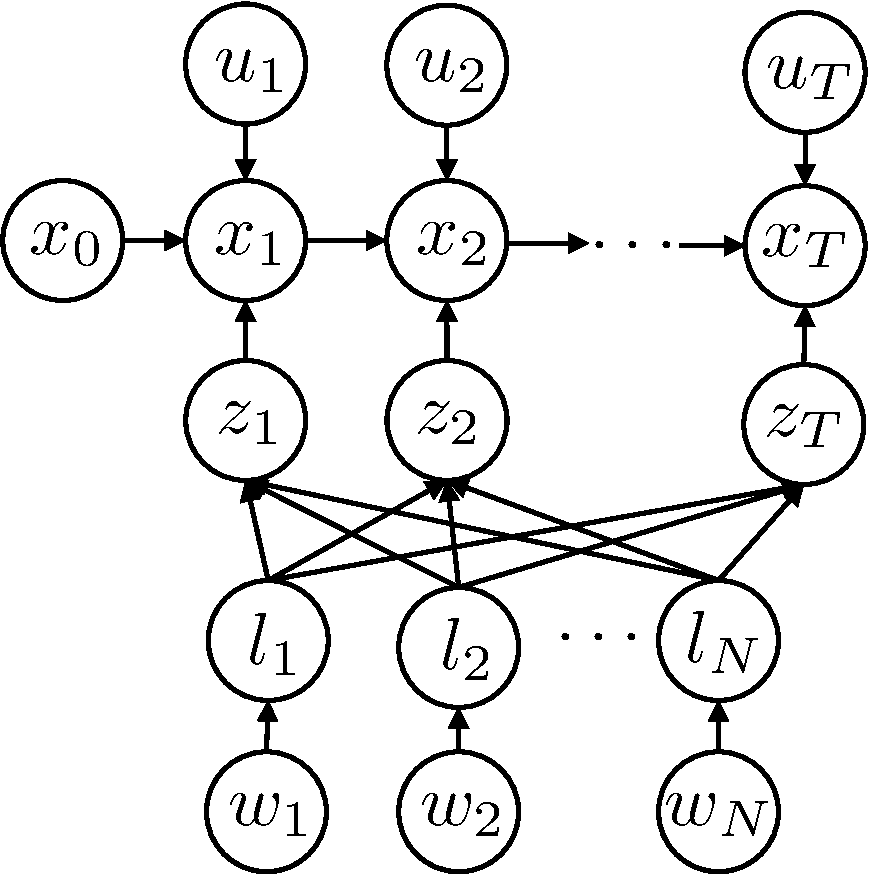
\includegraphics[width=0.5\columnwidth]{fig/model} 
\end{center}
\caption{Graphical Model Formulation. Dark nodes are observed.}
\label{fig:model}
\end{figure}
%\end{wrapfigure}

Following \cite{isam} we formulate the SLAM problem in graphical models as in Figure \ref{fig:model}. Specifically, the robot states are denoted by $X = \{x_i\}$ with $i \in 0, \dots T$, the landmarks by $L = \{l_j\}$ with $j \in 1,\dots, N$, the control inputs by $U = \{u_i\}$ for $i \in 1,\dots, T$ and the landmark measurements by $Z = \{z_k\}$ with $k \in 1, \dots, K$. In addition to the classical graph SLAM formulation, we augment the representation of landmarks with latent parameters $W = \{w_j\}$ with $j \in 1, \dots, N$ \cj{is W for data associateion? if so, this should be stated explicitly}. Then the joint probability of all variables and measurements are given by

%\begin{equation}
\begin{multline}
P(X, L, U, Z, W) \propto  \\
\prod\limits_{i}P(x_i|x_{i-1}, u_i)\prod\limits_{k}P(z_k|x_{i_k}, l_{j_k}, w_{j_k}).
\label{eq:jointProb}
\end{multline}
%\end{equation}

Then the maximum likelihood (ML) estimate of the unobserved poses $X$ and landmarks $L$ given observations $Z$, known controls $U$, and the current latent parameters $W$ is

\begin{equation}
X^*, L^* = \operatorname*{arg\,max}_{X,L} P(X,L,U,Z,W).
\end{equation}

To calculate the ML estimate, the objective is linearized and converted into a linear least
squares problem in this form $\operatorname*{arg\,min}_{\delta} || A
\delta  - b ||^2$ by algebraic manipulation, and then optimized using
different numerical methods. Derivation with more details is provided in appendix \ref{appendix:leastsquare}.

Using a Gaussian representation with the latent extension, the sensor
model, the process model and measurement equation follows

\begin{equation}
\begin{aligned}
x_i &= f_i(x_{i-1}, u_i) + \omega_i \\
z_k &= h_k(x_{i_k}, l_{j_k}) + \nu_k
\end{aligned}
\label{eq:gaussRepresentation}
\end{equation}

where $\omega_i$ and $\nu_k$ are noise terms which follow zero-mean normal distribution with covariance matrices $\Gamma_i$ and $\Sigma_k$. With this formulation, the second part of the joint probability \ref{eq:jointProb} is augmented with the mobility indicator. In addition we also apply a robust kernel to the observation term, then the formulation as a whole is given as:

\cj{need to reformat exp() to be within margin, e is placeholder}
%\begin{equation}
\begin{multline}
P(z_k|x_{i_k}, l_{j_k}, w_{j_k})\propto \\
 e^{(-w_{j_k} (v_k(z_k - h_k(x_{i_k}, l_{j_k})))^T \Sigma_k^{-1} (v_k(z_k - h_k(x_{i_k}, l_{j_k}))) }.
 %\exp(-w_{j_k} (v_k(z_k - h_k(x_{i_k}, l_{j_k})))^T \Sigma_k^{-1} (v_k(z_k - h_k(x_{i_k}, l_{j_k}))) ).
\label{eq:sensor}
\end{multline}
%\end{equation}

where $w_{j_k}$ is associated with each landmark representing the likelihood that the measurement comes from static landmark, and $v_k$ is the robust scaling factor associated with each landmark observation representing whether the measurement is an inlier. When $w_{j_k}$ or $v_k$ approaches zero, the effect is equivalent to making the covariance of the Gaussian very large, effectively rendering the distribution uniform and the constraint represented by the distribution of no impact on the graph optimization process. Note that $w_{j_k}$ can be negative because the formulation given here is proportional to a normalizing constant.
% In our case, we need to infer what their values are and ideally whether the process could be online or folows an incremental fashion. Possible solutions could be 1) using visual cues to cluster the landmarks to ``moving''/``static''. Challenges mainly lies in whether the features we use is reliable or not in terms of this clustering task; 2) instead of using an expensive EM algorithm in \cite{rogers2010slam}, we design particle filters to incrementally update parameter $w_k$, making the whole process online.

\section{EXPERIMENTS}

\begin{figure*}[!ht]
\makebox[\textwidth][c]{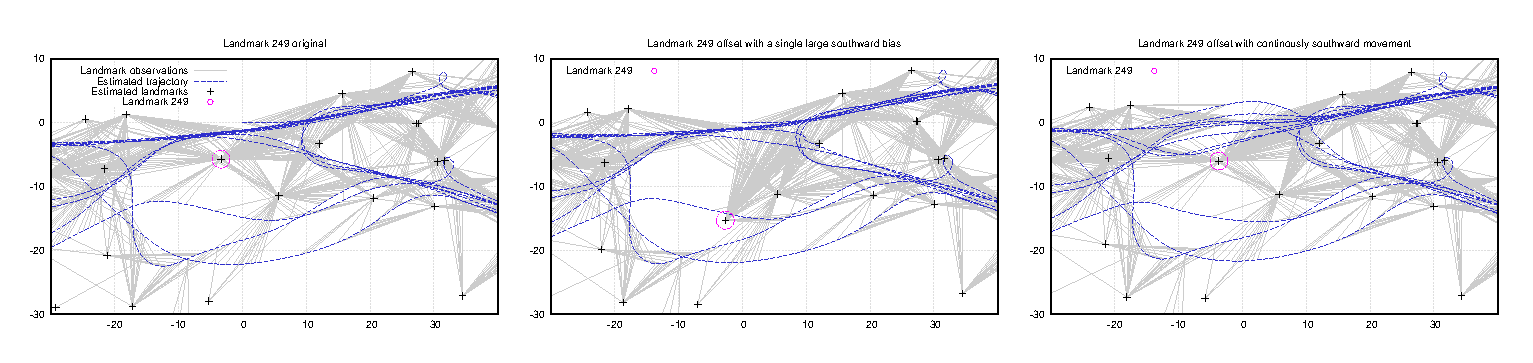
\includegraphics[width=\textwidth]{fig/baseline-mm}}
\caption{The optimal estimates of the trajectory and landmark positions
obtained by Max-Mixture graph SLAM.  Left: low convergence uncertainty
(measured by objective value). Middle: high convergence uncertainty because of
rejection of outlier observations of landmark 249.  Right: low convergence
uncertainty, no outlier detected by Max-Mixture.}
\label{fig:baseline}
\end{figure*}

We implemented our method as discussed previously and compared the result with
various alternative approaches. Our implementation is based on the graph
optimization framework g2o \cite{g2o}, and we programmed a plug-in type library
in C++ to represent our modified objective function while reusing the Gauss-Newton
optimization functionality. The type library exposes properties of the edges including
the error metric, reweighted information matrix, and robust Mahalanobis distance function.

\subsection{Datasets}

We use the commonly compared dataset Victoria Park released with iSAM
\cite{isam} and apply different types of simulated corruption to the dataset to
generate multiple synthesized datasets to evaluate the effect on different
approaches.  For the purpose of evaluating performance against moving
landmarks, several other commonly used datasets are not suitable because they
are pose-only graphs without landmarks. The Victoria Park dataset of 2-D
odometry and landmark observations contains 6969 robot poses, 6968 odometry
measurements, 151 landmarks, and 3640 landmark measurements obtained.

\subsection{Prior Methods with Moving Landmarks}

In this test, we evaluate the performance of the state-of-the-art robust
SLAM method, the Max-Mixture algorithm, given dynamic landmark measurements.
Max-Mixture is a robust extension to classical graph SLAM using Gaussian
mixture in factor representation, that is, $ x_i = \sum_c \phi_c
\mathcal{N}(\mu_c, \Sigma_c)$ for component $c$ and weight $\phi_c$, with
observations being components, also similarly for $z_i$. Max-Mixture uses a max
function to approximate and efficiently evaluate the sum of Gaussians. It is
well-known for its capability of handling a large amount of incorrect loop
closures, but it is untested against moving landmarks, and this experiment can
be representative to other approaches in the robust SLAM literature. 

We apply different perturbations to all observations associated with a certain
landmark which has the most observations associated in the dataset, and study
the different effects of the perturbations on the optimal estimate of the
trajectory and the map of all landmarks obtained by Max-Mixture graph SLAM. The
Victoria Park dataset contains 2-D odometry and landmark observations. As shown
in figure \ref{fig:baseline} the left plot is the control group without
perturbation, and is accurate to the ground truth. A single southward bias is
applied to all observations of the landmark in the middle plot, simulating
sensory outliers. A temporally increasing bias is applied to all observations
of the landmark in the right plot, simulating a southward moving landmark.

As the middle plot shows, Max-Mixture is still capable of handling noise of
large bias or spurious loop closures introduced by simulated sensory fault. It
correctly rejects outlier landmark observations and recovers the position of
the perturbed landmark. However, it completely fails to reject any unlikely
landmark observations and largely distorts the resulting trajectory when given
moving landmark measurements. An explanation for this is that each clique of
landmarks with coherent motion forms a plausible reference frame for related
observations. Inference based on each independent reference frame will reach
plausible estimate of robot trajectory and the map, however robust SLAM methods
which assume stationary landmarks will average over a sum of different
reference frames and lead to wrong conclusions.

\subsection{Our Method Compared with Prior Methods}

To benchmark the robustness of the proposed approach and to show its
correctness and feasibility, we use the Victoria Park dataset that has been
used in a number of publications before. The dataset consists of pose graphs in
2D and contain several thousand poses and landmark constraints. We corrupted
the data by setting landmark ``249" (circled in red) in a constant northward
movement, where its eventual position is roughly 7 meters north of its original
location. We chose landmark ``249" due to the relatively large amount of
observations associated with this particular landmark in the dataset. We expect
the more observations there are on a landmark, the greater its movement would
corrupt the final optimization results and the more possible that existing
robust SLAM methods would fail.

We compare the results of Dynamic Covariance Scaling robust kernel as discussed in our
formulation, and also the SLAM with EM approach proposed in \cite{rogers2010slam}.

\begin{figure}[ht]
\centering
\begin{minipage}[b]{0.48\textwidth}
  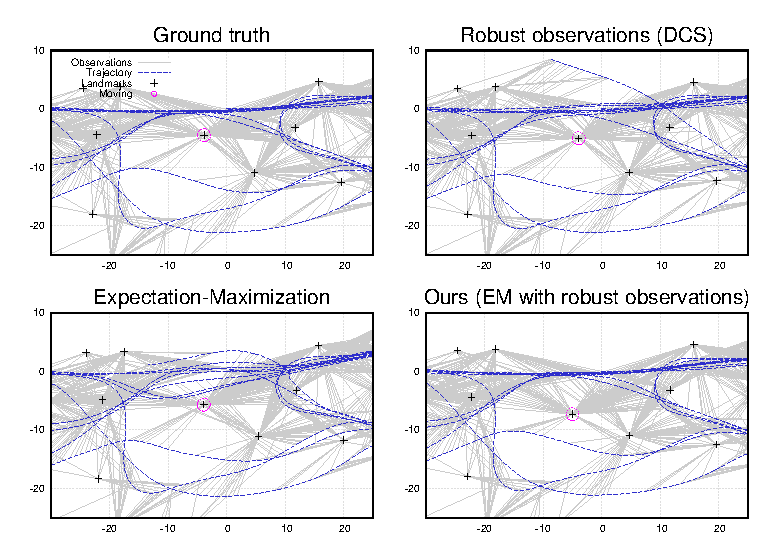
\includegraphics[width=\textwidth]{fig/small-movement}
  \caption{Dataset corrupted by the landmark with small movement}
  \label{fig:small-movement}
\end{minipage}
\quad
\begin{minipage}[b]{0.48\textwidth}
  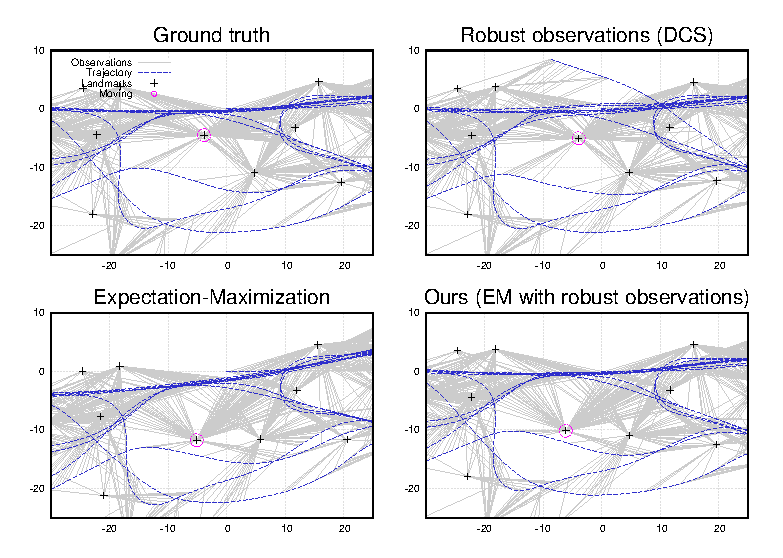
\includegraphics[width=\textwidth]{fig/large-movement}
  \caption{Dataset corrupted by the landmark with large movement}
  \label{fig:large-movement}
\end{minipage}
\end{figure}

Figure \ref{fig:small-movement} shows the results for DCS, normal EM, and our
approach. As shown in the figure, robust observations alone are unable to
handle moving landmarks. This is because observation based robust methods do
not characterize the mobility of the landmark and its effect on associated
observations and assume independence between observations which is not the case
for moving landmarks. A moving landmark will cause associated observations to
be inconsistent in a plausible way such that a subgroup of the observations
might be able to converge to a local minimum but the rest of the observations
would distort the result elsewhere. 

Normal SLAM with EM was proposed in \cite{rogers2010slam} for datasets with
very large movement. Their formulation is similar with ours except it is
without the robust factor $v_k$.  As shown in figure \ref{fig:small-movement},
the resulting trajectory is distorted. One explanation for this is from the
charactersstics of the datasets.  In their paper, they investigated datasets
containing landmarks moved from one room to another room over a long period of
time, which is not the case in the dataset presented in figure
\ref{fig:small-movement} where the motion of the landmark is relatively small
and continuous. In fact, in figure \ref{fig:large-movement} the motion of the
corrupted landmark is doubled and normal EM is able to learn the mobility
correctly.

Our robust back-end however, is able to converge to a correct solution in a few
iterations. Our result is also verified by examining the learned parameters
$w_{j_k}$ and $v_k$ of all landmarks, which is close to zero for the actual
outlier landmarks, thus correctly deactivating associated corrupted
observations.  The improvement is explained by our utilization of the robust
kernel to make the EM algorithms reliably learn the mobility indicators of the
landmarks correctly identify the actual moving landmarks. Thus our approach is
able to obtain the best results in both situations.

%\begin{wrapfigure}{r}{0.25\textwidth}
\begin{figure}
\begin{center}
%\framebox[4.0in]{$\;$}
%\fbox{\rule[-.5cm]{0cm}{4cm} \rule[-.5cm]{4cm}{0cm}}
 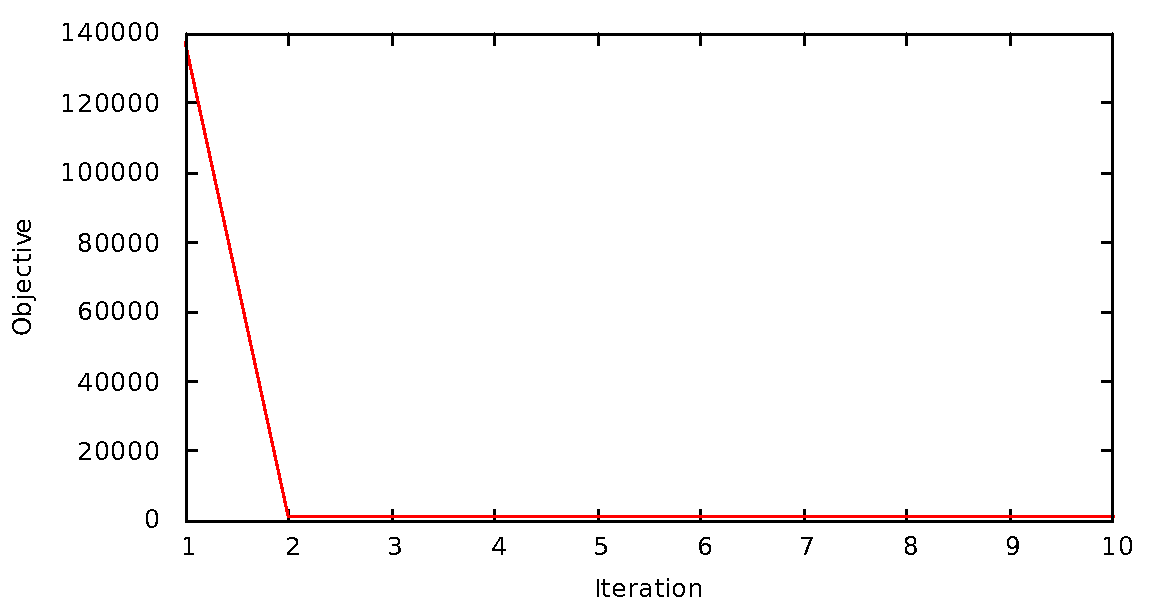
\includegraphics[width=0.8\columnwidth]{fig/objective}
\end{center}
\caption{Learning objective versus iterations}
\label{fig:objective}
\end{figure}
%\end{wrapfigure}

To help verify our learning algorithm, we also provide the plot of our learning
objective versus learning iterations in the right figure \ref{fig:objective}.
The algorithm almost converges after 2 iterations, mostly because the number of
outliers introduced is relatively small compared to the total number of
landmarks, and the graph optimization step eliminates the majority of the
energy besides that caused by wrong identification of landmark mobility.

\section{Discussion}

Inference challenges need to be solved: 1) Not fast enough, how to make EM fast? How to decompose the EM problem into incremental parts? 2) Not robust enough, need testing with real world and see failure modes.

An experimental evaluation protocol: most data related to SLAM will or should have ground truth. To evaluate, compare with the ground truth to determine if  the result is accurate enough. Examine the internals of EM, log-likelihood of each iteration, chi-square test to verify the internal correctness.

\section{Timeline}

\bibliographystyle{plain}
\bibliography{cs242_slam}
%\subsection{Figures}
%\begin{figure}[h]
%\begin{center}
%%\framebox[4.0in]{$\;$}
%\fbox{\rule[-.5cm]{0cm}{4cm} \rule[-.5cm]{4cm}{0cm}}
%\end{center}
%\caption{Sample figure caption.}
%\end{figure}

\end{document}
